\section{Cross Section}
\label{sec:AN_CrossSection}

The cross section of $pp\rightarrow W\gamma \rightarrow l\nu\gamma$, where $l=\mu,e$, is measured following the procedure described in Ch.~\ref{sec:AN_WgMeasStrategy} based on CMS data at $\sqrt{s}=$8~TeV in the phase space defined in the beginning Ch.~\ref{sec:AN_WgMeas}. The measured cross section is compared to the phase-space-corrected MCFM calculation at NLO which is referred to as ``NLO theory''.  

The cross section of the $W\gamma$ production was computed with MCFM at NLO with the phase space constraints at which the simulated $W\gamma$ sample was produced. The NLO cross section equals to $\sigma_1=$554~pb. NNLO and higher order corrections are expected to have an effect of $\~$20\%. 

The cross section in our selected phase space was computed as 
\begin{center}
$\sigma_2 = \sigma_1 \cdot \frac{N_2}{N_1}$, 
\end{center} 
\noindent{where  $N_2$ and $N_1$ are the total MC sample event count and event count in the phase space of this measurement, respectively. For the differential cross section, $N_2$ is number of events falling into specific $P_T^{\gamma}$ bin, and to compute $\frac{d\sigma }{ dP_T^{\gamma}}$, we divide the cross section by the bin width.}

%\begin{center}
%\frac{{d\sigma }{ dP_T^{\gamma}}}, 
%\end{center} 
%\noindent{we divide by the bin width.} 

The total measured cross section in the muon and electron channel is \\
%$\sigma(W\gamma\rightarrow\mu\nu\gamma)=10949 \pm 91$ (stat.) $ \pm 2959$ (syst.) fb\\
\begin{center}
$\sigma(W\gamma\rightarrow\mu\nu\gamma)=$11040$\pm$91(stat.)$\pm$2954(syst.)~fb\\
$\sigma(W\gamma\rightarrow\mu\nu\gamma)=$9146$ \pm $185(stat.)$\pm$3981(syst.)~fb\\
\end{center}
The corresponding NLO theory value is 9101~fb.

% ADD THEORY VALUE

Table~\ref{tab:cs_mc_vs_meas_WGamma} and Fig.~\ref{fig:CS_Wg} summarize the results of the differential cross section. Because we applied the detector resolution unfolding procedure, the measurements in different $P_T^{\gamma}$ bins are correlated. Correlation matrices provided in Ch.~\ref{sec:Unfolding} and App.~\ref{sec:corrMatrices} are correlation matrices on unfolded yields. The uncertainties provided in the Tab.~\ref{tab:cs_mc_vs_meas_WGamma} and Fig.~\ref{fig:CS_Wg} are diagonal elements of the error matrices.

The measured cross sections in different channels agree between each other as well as with the NLO theory cross section provided uncertainties of the measured cross section. The systematic uncertainties on the measured cross section are dominant over the statistical uncertainties. In the muon channel and in $P_T^{\gamma}<$55~GeV bins of the electron channel, the most significant sources of the sytematic uncerntainty are sources associated with jets$\rightarrow\gamma$ background estimation. In high $P_T^{\gamma}$ bins of the electron channel, uncerntainties on photon efficiency scale factors become more significant.

For validation of the measurement procedure, we measure the cross section of $Z\gamma$ and compare the result with the published CMS result for $Z\gamma$ at~8~TeV. We measure the cross section in the muon and electron channels in the same phase space as the published CMS measurement~\cite{ref_Zg8TeV}. 

$Z\gamma\rightarrow\mu\mu\gamma$ FSR and ISR datasets which are used to prepare real-$\gamma$ and fake-$\gamma$ templates for jets$\rightarrow\gamma$ background estimation largely overlap with nominally selected $Z\gamma$ dataset. Therefore, the measurement of $Z\gamma$ cross section in the muon channel is a closure check while the measurement of $Z\gamma$ cross section in the electron channel is a fully valid physics measurement. The results of our $Z\gamma$ measurement agree well with the published results as well as with the theory predictions, and the systematic uncertainties on our $Z\gamma$ measured cross section are much smaller than on our $W\gamma$ measured cross section. The details of the $Z\gamma$ check are available in App.~\ref{sec:ZgCheck}.

The ongoing $W\gamma$ measurement based on~2015 and~2016 datasets has higher chances to discover a potential new physics because of higher energy of $\sqrt{s}=$13~TeV and higher statistical power of over~30~fb$^{-1}$. Although the largest uncertainties of the~8~TeV measurement are systematic uncertainties, many of them depend on amount of data in control samples, thus, the increased size of the data sample will help to reduce those uncerntainties. Higher collision energy allows us to observe more signal events in high $P_T^{\gamma}$ ranges where the effect of potential aTGC is the largest. 

\begin{table}[h]
  \scriptsize
  \begin{center}
  \caption{Cross section and uncertainties. The first uncertainty is statistical and the second one is systematic.}
  \begin{tabular}{|c|c|c|c|}
                     & \multicolumn{3}{|c|}{$d\sigma/dP_{T}^{\gamma}$, fb/GeV} \\ 
     $P_T^{\gamma}$, & NLO theory                          &  \multicolumn{2}{|c|}{measured}      \\
    GeV              &  $W\gamma\rightarrow l\nu\gamma$ & $W\gamma\rightarrow \mu\nu\gamma$  & $W\gamma\rightarrow e\nu\gamma$    \\ \hline
%    total & 9101 & 11040 $\pm$ 91 $\pm$ 2954 & 9146 $\pm$ 185 $\pm$ 3981 \\ \hline
%    10-15 & 1548 & 1771 $\pm$ 33 $\pm$ 274 & 889 $\pm$ 40 $\pm$ 691\\ \hline
    15-20 & 751 & 751 $\pm$ 17 $\pm$ 257 & 440 $\pm$ 35 $\pm$ 396\\ \hline
    20-25 & 378 & 422 $\pm$ 10 $\pm$ 145 & 338 $\pm$ 23 $\pm$ 163\\ \hline
    25-30 & 210 & 292 $\pm$ 7 $\pm$ 86 & 298 $\pm$ 16 $\pm$ 107\\ \hline
    30-35 & 129 & 177 $\pm$ 5 $\pm$ 80  & 193 $\pm$ 9 $\pm$ 82\\ \hline
    35-45 & 70 & 122 $\pm$ 2 $\pm$ 23 & 103 $\pm$ 3 $\pm$ 29\\ \hline
    45-55 & 35 & 35 $\pm$ 1 $\pm$ 23 & 34 $\pm$ 3 $\pm$ 24\\ \hline
    55-65 & 22 & 31 $\pm$ 1 $\pm$ 8  & 31 $\pm$ 2 $\pm$ 18\\ \hline
    65-75 & 14 & 16 $\pm$ 1 $\pm$ 7 & 19 $\pm$ 1 $\pm$ 12 \\ \hline
    75-85 & 9 & 16 $\pm$ 1 $\pm$ 3 & 12 $\pm$ 1 $\pm$ 8\\ \hline
    85-95 & 6.4 & 9.9 $\pm$ 0.5 $\pm$ 2.4 & 10.0 $\pm$ 0.9 $\pm$ 4.3\\ \hline
    95-120 & 3.7 & 6.0 $\pm$ 0.3 $\pm$ 1.0 & 4.9 $\pm$ 0.4 $\pm$ 2.5\\ \hline
    120-500 & 0.27 & 0.43 $\pm$ 0.01 $\pm$ 0.10 & 0.46 $\pm$ 0.02 $\pm$ 0.22\\ \hline
  \end{tabular}
  \label{tab:cs_mc_vs_meas_WGamma}
  \end{center}
\end{table}
 
\begin{figure}[htb]
  \begin{center}
   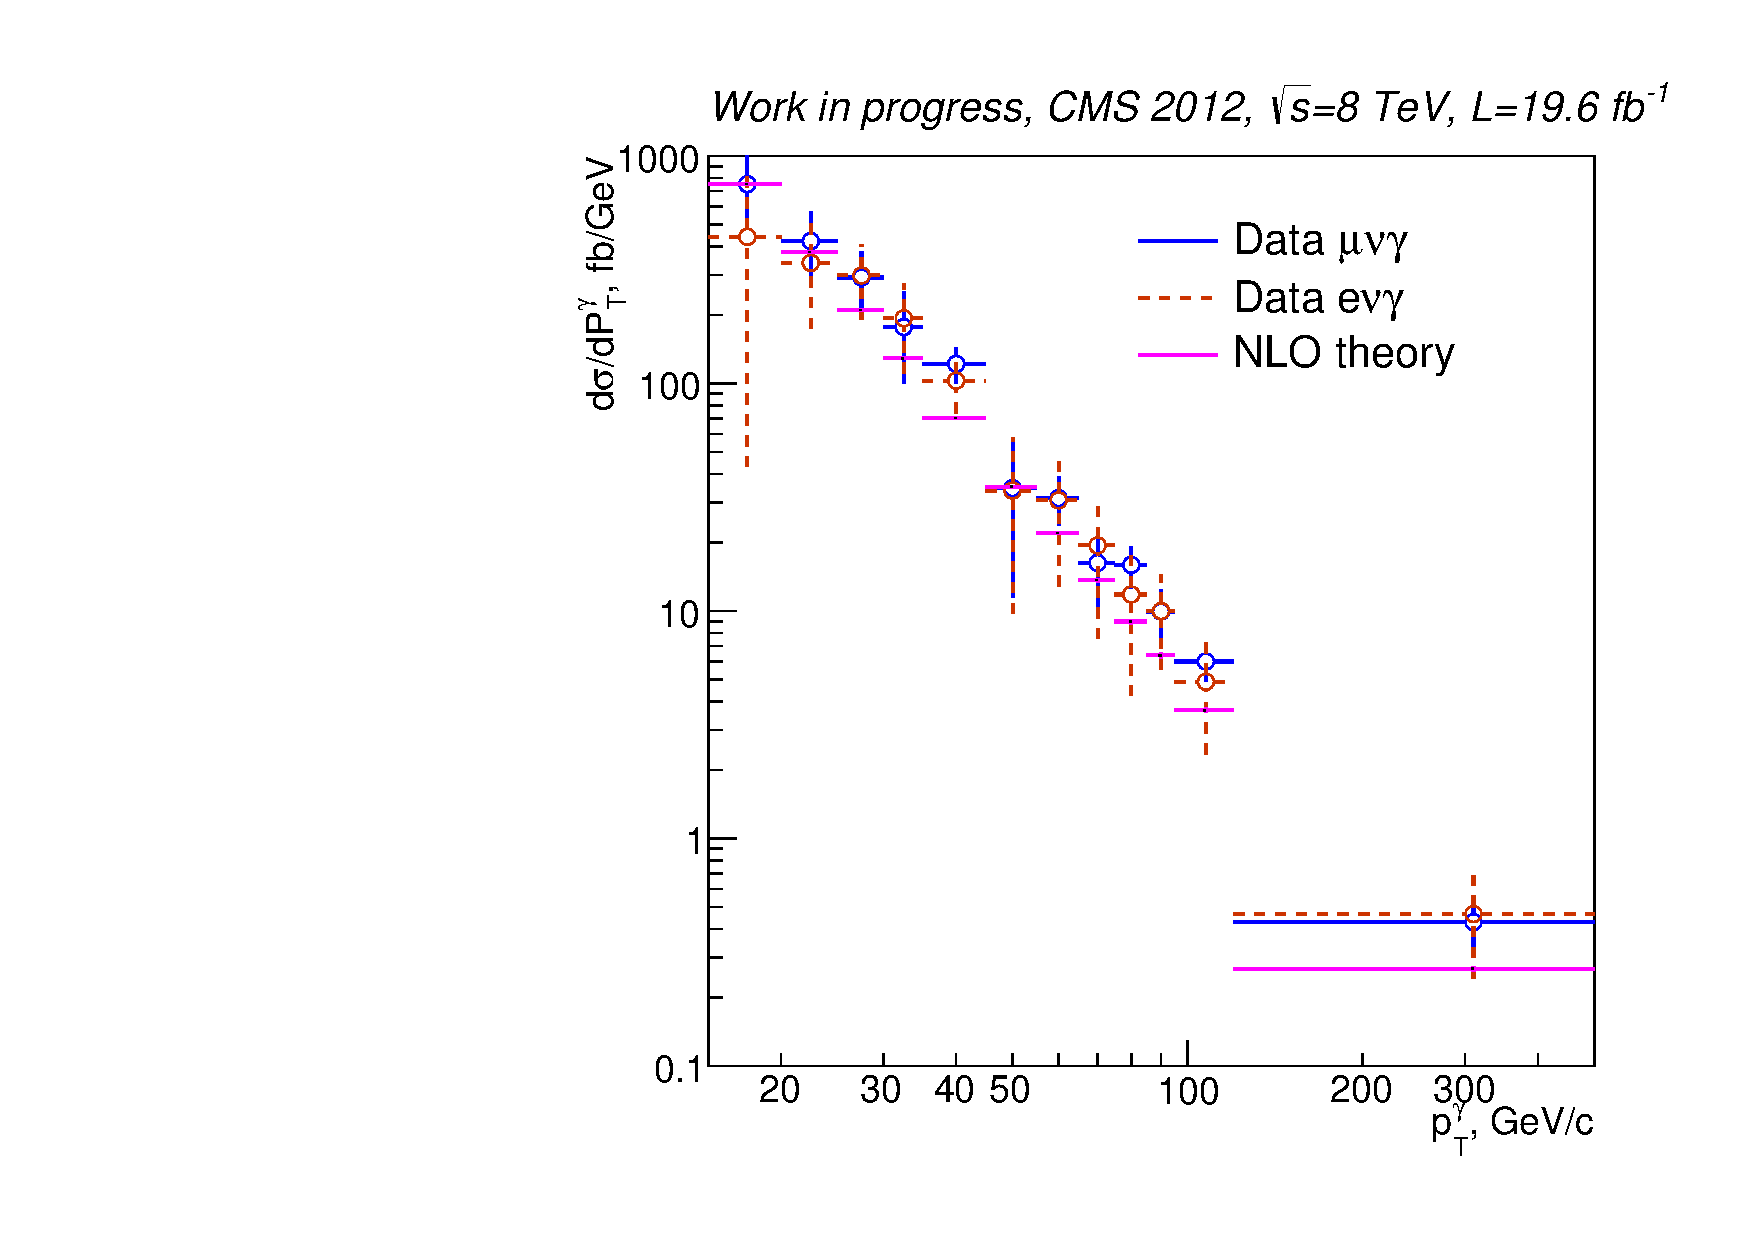
\includegraphics[width=0.5\textwidth]{../figs/figs_v11/ChannelsMERGED_WGamma/CrossSection/compareCSWGamma.pdf}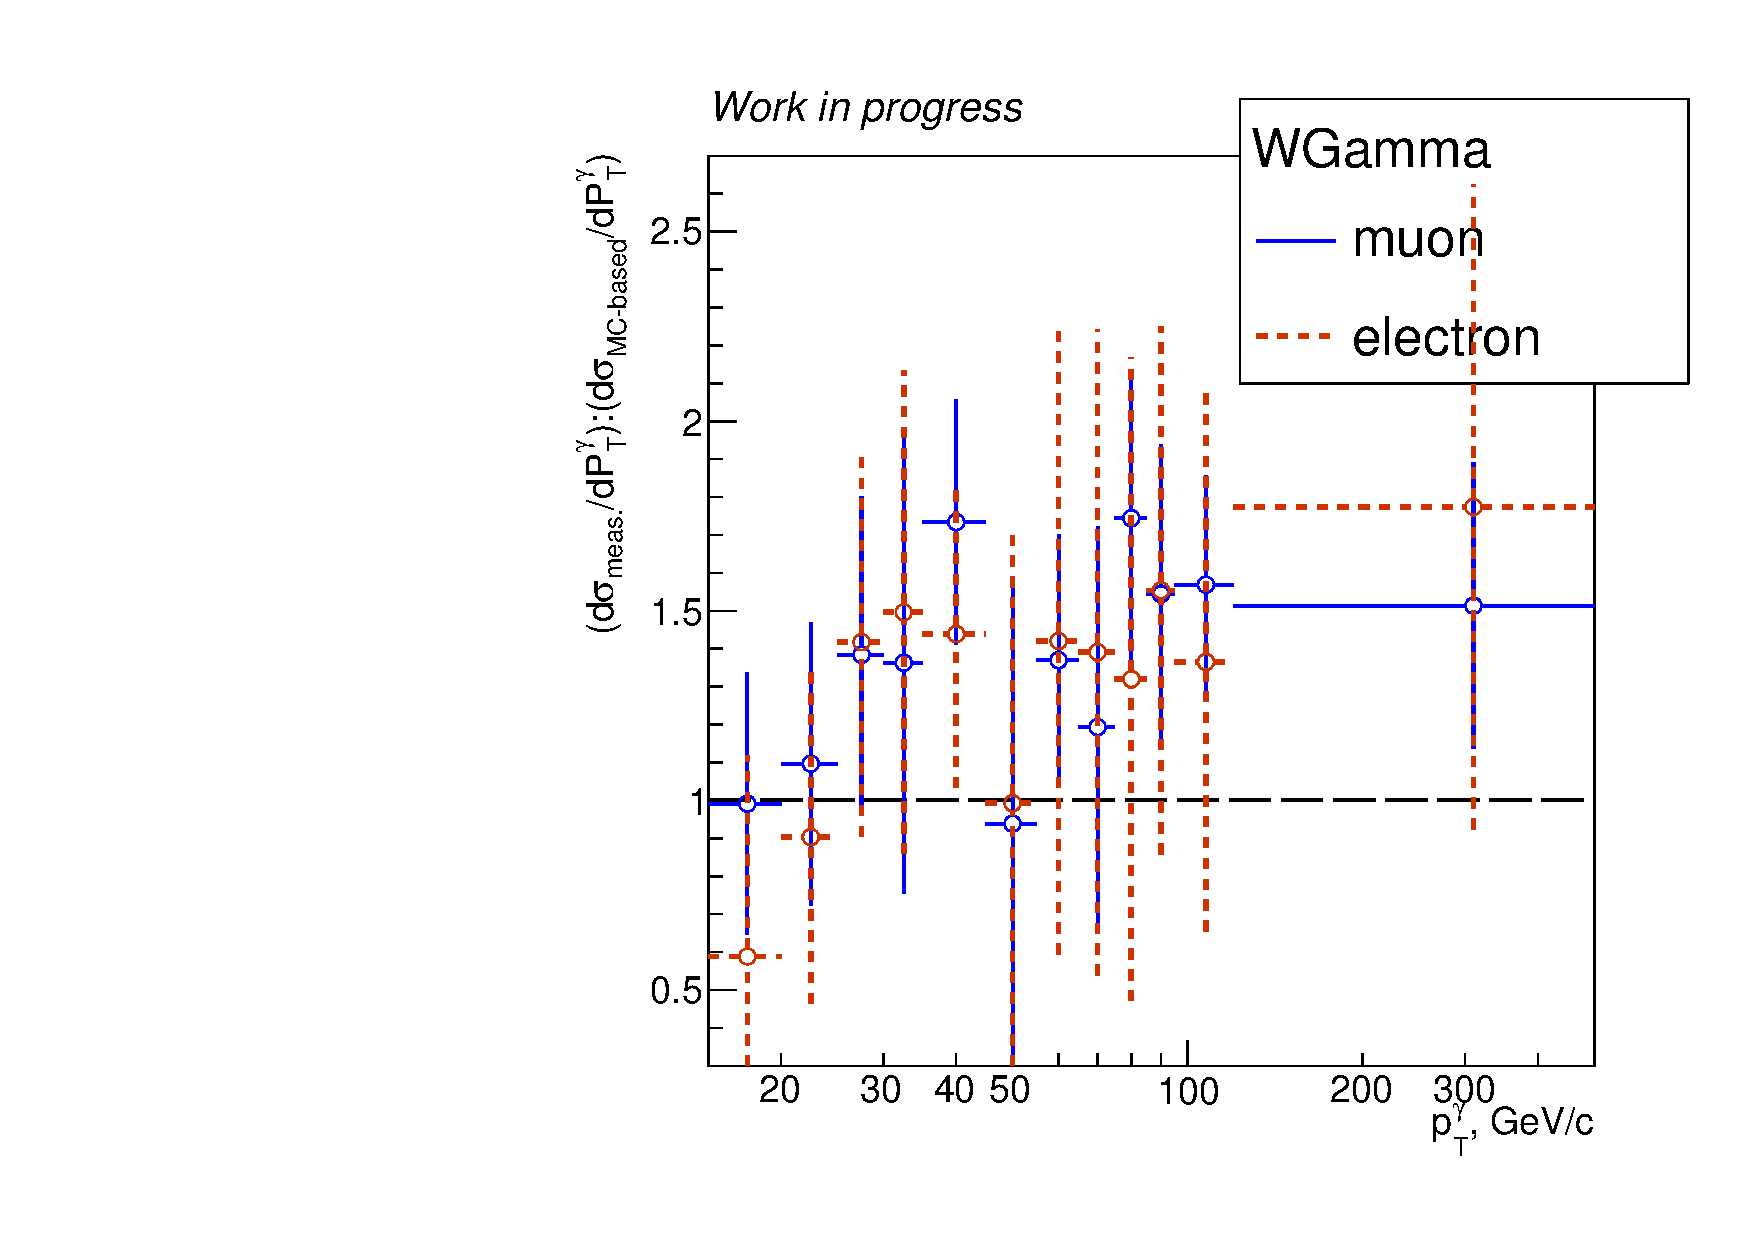
\includegraphics[width=0.5\textwidth]{../figs/figs_v11/ChannelsMERGED_WGamma/CrossSection/compareCSratioTheoryWGamma.pdf}
  \caption{Left: the differential cross section of the $W\gamma$ production $d\sigma/dP_T^{\gamma}$; right: the ratio between the measured and the NLO theory differential cross section of the $W\gamma$ production. }
  \label{fig:CS_Wg}
 \end{center}
\end{figure}
